\documentclass[a4paper]{llncs}
\usepackage[latin1]{inputenc}
\usepackage{amsmath}
\usepackage{amssymb}
\usepackage[algo2e]{algorithm2e}
\usepackage{pgf}
\usepackage{tikz}
\usepackage{verbatim}
\usetikzlibrary{arrows,automata}
\usepackage{graphicx}
\usepackage{sidecap}
%% \usepackage{caption}
\usepackage{subcaption}

\usepackage{url}
\urldef{\mailsa}\path|cs1090197@cse.iitd.ac.in|

\setcounter{tocdepth}{3}

\begin{document}

\mainmatter

\title{Tools and Algorithms for Deciding Relations on Timed Automata}

\author{Mihir Mehta}

\institute{Department of Computer Science and Engineering,\\
  Indian Institute of Technology, Delhi.\\
  \mailsa\\
}

%% \date{April 2013}

\maketitle

\begin{abstract}
  This describes the author's work in implementing the construction of
  zone-valuation graphs for timed automata and using these to verify
  certain relations on pairs of timed automata.
\end{abstract}
\pagebreak

\tableofcontents
\pagebreak
\listoffigures
\listoftables
\pagebreak

\section{Objectives}

The work described in this thesis builds on the work of
\cite{DBLP:conf/cav/GuhaNA12} in which Guha et al described an
algorithm to generate \emph{zone valuation graphs} for timed automata
and an algorithm to use such zone-valuation graphs to determine
\emph{timed performance prebisimilarity} on pairs of timed
automata. Our aim was to implement these algorithms in a generalised
manner in order to verify various other time abstracted relations,
such as time abstracted bisimulations \cite{tripakis2001analysis} and
time abstracted simulation equivalence. Towards
this end, we studied the literature about timed
untimed automata as well as various existing tools for verifying these
equivalences (such as \texttt{minim}, described in
\cite{tripakis2001analysis}). Our implementation, in OCaml, implements
several of these relations and leaves some scope for implementing others.

\section{Labelled transition systems}

\begin{SCfigure}
  \centering
  \def\svgwidth{0.3\columnwidth}
  \input{lts01.pdf_tex}
  \caption{An example of a labelled transition system. Here, the
    states are $\{0, 1, 2, \ldots 7\}$ and the actions are $\{0,
    1\}$.}
  \label{lts01}
\end{SCfigure}

\begin{definition}
  \emph{Labelled Transition System}: A labelled transition system (LTS)
  \cite{Keller:1976:FVP:360248.360251} is an automaton which is
  described by
  \begin{itemize}
  \item $S$, a set of \emph{states} 
  \item $Act$, a set of \emph{actions}
  \item $\rightarrow \subseteq S \times Act \times S$, a \emph{transition
    relation}.
  \item optionally, $I \subseteq S$ ,a set of initial states.
  \end{itemize}
\end{definition}

LTS are useful for describing the behaviour of untimed systems, and
serve as the foundation for the development of more complex models
such as CCS and timed automata. Thus, equivalences on LTS serve
as the theoretical foundation for many timed and time abstracted
equivalences on timed automata, and also have direct applications in
determining some of these equivalences in cases where timed automata
can be reduced to equivalent LTS.

\section{Equivalences on labelled transition systems}

\subsection{Strong bisimilarity}

\begin{SCfigure}
  \centering
  \def\svgwidth{0.5\columnwidth}
  \input{lts01quotient.pdf_tex}
  \caption{Strong bisimilarity quotient of the LTS in Figure~\ref{lts01}.}
\end{SCfigure}

\begin{definition} 
  \emph{Strong bisimulation}: A binary relation $R$ is a \textit{strong
    bisimulation} if and only if, for all $(s_1, s_2)$ $\epsilon$ $R$ and $a$ $\epsilon$ $Act .$\\
  $\forall s_1' (s_1 \xrightarrow{a} s_1' \Rightarrow \exists s_2'
  . (s_2 \xrightarrow{a} s_2' \wedge (s_1', s_2')$ $\epsilon$ $R ) )
  \wedge $ \\
  $\forall s_2' (s_2 \xrightarrow{a} s_2' \Rightarrow \exists s_1'
  . (s_1 \xrightarrow{a} s_1' \wedge (s_1', s_2')$ $\epsilon$ $R ) )$
\end{definition}

\begin{definition}
  \emph{Strong bisimilarity}: It can be shown that the union of
  all strong bisimulations over the set of states is a strong
  bisimulation. This binary relation is called \textit{strong
    bisimilarity}, denoted by $\sim$.
\end{definition}

\section{Timed automata}

\begin{SCfigure}
  \centering
  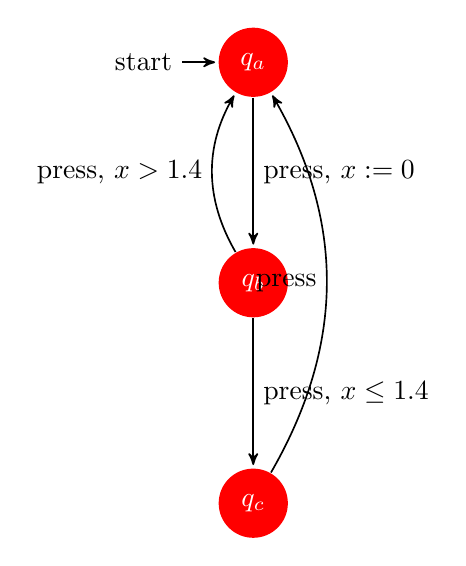
\begin{tikzpicture}[->,>=stealth',shorten >=1pt,auto,node
      distance=2.8cm,
      semithick]
    \tikzstyle{every state}=[fill=red,draw=none,text=white]

    \node[initial,state] (A)                    {$q_a$};
    \node[state]         (B) [below of=A] {$q_b$};
    \node[state]         (C) [below of=B] {$q_c$};
    
    \path (A) edge              node {press, $x:=0$}    (B)
    (B) edge [bend left] node {press, $x > 1.4$}        (A)
    edge              node {press, $x \le 1.4$}         (C)
    (C) edge [bend right] node {press}                  (A);
  \end{tikzpicture}

  \caption{Timed automaton representing a light bulb with two
    brightness settings, example taken from \cite{aceto2007reactive}}
\end{SCfigure}

\begin{definition}
  \emph{Timed Automaton}: timed automaton over a finite set of clocks $C$
  and a finite set of actions $Act$ is a 4-tuple $(L, l_{0}, E, I)$.
  \begin{itemize}
  \item $L$ is a finite set of locations.
  \item $l_{0}$ is the initial location.
  \item $E \subseteq L \times B(C) \times Act \times 2^{C} \times L$
    is a finite set of edges.
  \item $I: L \rightarrow B(C)$ assigns invariants to each edge
    location.
  \item $B(C)$ is the set of clock constraints over C. An element of $B(C)$
    can be an equality, a slack inequality, or a strict inequality on
    $v(x)$ for some $x$ $\epsilon$ $C$, or
    an AND combination of such constraints.
  \item The state of the automaton at any particular instant is given
    by the ordered pair $(l, v)$ which gives the location and assigns
    a value to each clock. 
  \item A transition is either a delay transition where the automaton
    stays at the same location while advancing each clock by the same
    time delay, or an action transition where the automaton performs a
    state change while resetting some of its clocks.
  \end{itemize}
\end{definition}

It is evident that the state space in a timed automaton is, in
general, uncountably infinite. This makes it impossible for any
algorithm to terminate which explores the state space in a naive
manner. However, some standard techniques to discretise the state
space of timed automata exist, which we elaborate on, below.

\begin{itemize}

\item \emph{State}: A state of a timed automaton is a pair $(l, v)$
  where $l$ is a location in the automaton and $v$ is a clock
  valuation satisfying $l.invar$

\item \emph{Symbolic state}: A symbolic state is a set of states in
  the timed automaton. The constituent states do not necessarily share
  a location.

\item \emph{Zone}: A zone is a symbolic state where the all the
  constituent states share a location and the set of valuations of
  these states forms a convex polyhedron on the valuation space.

\end{itemize}

\section{Timed relations on timed automata}

\subsection{Time abstracted bisimilarity}

\begin{definition}  
  \emph{Strong time abstracted bisimulation}: A binary relation
  $R$ is a strong time abstracted bisimulation (STaB) if and only if, for all
  $(s_1, s_2)$ $\epsilon$ $R$ , $a$ $\epsilon$ $Act $, $d$ $\epsilon$ $R_{\ge 0}$\\
  $\forall s_1' (s_1 \xrightarrow{a} s_1' \Rightarrow \exists s_2'
  . (s_2 \xrightarrow{a} s_2' \wedge (s_1', s_2')$ $\epsilon$ $R ) )
  \wedge $ \\
  $\forall s_2' (s_2 \xrightarrow{a} s_2' \Rightarrow \exists s_1'
  . (s_1 \xrightarrow{a} s_1' \wedge (s_1', s_2')$ $\epsilon$ $R ) ) \wedge $ \\
  $\forall s_1' (s_1 \xrightarrow{d} s_1' \Rightarrow \exists (s_2',
  d')
  . (s_2 \xrightarrow{d'} s_2' \wedge (s_1', s_2')$ $\epsilon$ $R ) )
  \wedge $ \\
  $\forall s_2' (s_2 \xrightarrow{d} s_2' \Rightarrow \exists (s_1', d')
  . (s_1 \xrightarrow{d'} s_1' \wedge (s_1', s_2')$ $\epsilon$ $R ) ) $ \\
\end{definition}

\begin{definition}
  \emph{Strong time abstracted bisimilarity}: It can be shown that the union of all strong time abstracted
  bisimulations over the set of (location, valuation) pairs is a
  strong time abstracted bisimulation. This binary relation is called
  \textit{strong time abstracted bisimilarity}.
\end{definition}

\begin{definition}
  \emph{Time abstracted delay bisimulation}: A binary relation
  $R$ is a time abstracted delay bisimulation (TadB) if and only if, for all
  $(s_1, s_2)$ $\epsilon$ $R$ , $a$ $\epsilon$ $Act $, $d$ $\epsilon$ $R_{\ge 0}$\\
  $\forall s_1' (s_1 \xrightarrow{a} s_1' \Rightarrow \exists (s_2', d)
  . (s_2 \xrightarrow{d} \xrightarrow{a} s_2' \wedge (s_1', s_2')$ $\epsilon$ $R ) )
  \wedge $ \\
  $\forall s_2' (s_2 \xrightarrow{a} s_2' \Rightarrow \exists (s_1', d)
  . (s_1 \xrightarrow{d} \xrightarrow{a} s_1' \wedge (s_1', s_2')$
  $\epsilon$ $R ) ) 
  \wedge $ \\
  $\forall s_1' (s_1 \xrightarrow{d} s_1' \Rightarrow \exists (s_2',
  d')
  . (s_2 \xrightarrow{d'} s_2' \wedge (s_1', s_2')$ $\epsilon$ $R ) )
  \wedge $ \\
  $\forall s_2' (s_2 \xrightarrow{d} s_2' \Rightarrow \exists (s_1', d')
  . (s_1 \xrightarrow{d'} s_1' \wedge (s_1', s_2')$ $\epsilon$ $R ) ) $ \\
\end{definition}

\begin{definition}
  \emph{Time abstracted delay bisimilarity}: It can be shown that the
  union of all time abstracted delay bisimulations over the set of
  (location, valuation) pairs is a time abstracted delay
  bisimulation. This binary relation is called \textit{time abstracted
    delay bisimilarity}.
\end{definition}

\begin{definition}
  \emph{Time abstracted observational bisimulation}: A binary relation
  $R$ is a time abstracted observational bisimulation (TaoB) if and only if, for all
  $(s_1, s_2)$ $\epsilon$ $R$ , $a$ $\epsilon$ $Act $, $d$ $\epsilon$ $R_{\ge 0}$\\
  $\forall s_1' (s_1 \xrightarrow{a} s_1' \Rightarrow \exists (s_2',
  d, d') . (s_2 \xrightarrow{d} \xrightarrow{a} \xrightarrow{d'} s_2'
  \wedge (s_1', s_2')$ $\epsilon$ $R ) ) \wedge $ \\
  $\forall s_2' (s_2 \xrightarrow{a} s_2' \Rightarrow \exists (s_1',
  d, d') . (s_1 \xrightarrow{d} \xrightarrow{a} \xrightarrow{d'} s_1'
  \wedge (s_1', s_2')$ $\epsilon$ $R ) ) \wedge $ \\
  $\forall s_1' (s_1 \xrightarrow{d} s_1' \Rightarrow \exists (s_2',
  d')
  . (s_2 \xrightarrow{d'} s_2' \wedge (s_1', s_2')$ $\epsilon$ $R ) )
  \wedge $ \\
  $\forall s_2' (s_2 \xrightarrow{d} s_2' \Rightarrow \exists (s_1', d')
  . (s_1 \xrightarrow{d'} s_1' \wedge (s_1', s_2')$ $\epsilon$ $R ) ) $ \\
\end{definition}

\begin{definition}
  \emph{Time abstracted observational bisimilarity}: It can be shown that
  the union of all time abstracted observational bisimulations over the
  set of (location, valuation) pairs is a time abstracted observational
  bisimulation. This binary relation is called \textit{time abstracted
    observational bisimilarity}.
\end{definition}

\section{Algorithms}

\subsection{Creation of the zone valuation graph}

\subsubsection{Overview}

This algorithm is adapted from the algorithms in
\cite{DBLP:conf/cav/GuhaNA12} and \cite{guha2013notes}. We changed it
to make the correctness more evident. 
This algorithm consists of a \emph{forward
  propagation} which ensures that all \emph{reachable} zones are created, and a
\emph{backward propagation} which ensures that each zone is \emph{stable} with
respect to its successors. \\

For the forward propagation, we use a queue,
akin to the queue of the classic \emph{breadth-first search} algorithm
for graphs, to traverse the timed automaton, starting from the inital
location, to ensure that all reachable zones are created. In each
queue element (with the exception of the first element containing the
inital location, which has no predecessor), we store a location
$l_{succ}$, its predecessor in the current path $l_{pred}$, and the
transition $t$ from $l_{pred}$ to $l_{succ}$. It should be noted
that this may result in some locations being visited multiple times,
and in unreachable locations never being visited. Each time a location
is visited, we create therein, new zones which are reachable from the
zones of the predecessor. \\
Thus, for each predecessor zone $(l_{pred}, \zeta _{pred_{i}})$, the
derived successor zone is $(l_{succ}, \zeta _{succ_{i}})$, where

\begin{displaymath} 
  \zeta _{succ_{i}} = ((\zeta _{pred_{i}} \uparrow \cap t.guard)[t.resets := 0]) \uparrow
\end{displaymath} 

Thus, if we let  $(l_{pred}, \zeta _{pred_{i}})$ range over the
existing zones of $l_{pred}$, and if we let  $(l_{succ}, \zeta
_{succ_{j}})$ range over the existing zones of $l_{succ}$, then the
new zones in $l_{succ}$ will cover

\begin{displaymath} 
  \zeta _{succ_{new}} = (\bigcup _{i} \zeta_{succ_{i}}) - (\bigcup _{j} \zeta_{succ_{j}})
\end{displaymath} 

Since $\zeta _{succ_{new}}$ is not necessarily convex, we may need to
split it into multiple convex polyhedra before creating the
corresponding zones in the $l_{succ}$. Then, we split the zones of
$l_{succ}$ to ensure stability with respect to
its invariant and outgoing edge constraints. If any new
zones are thus created, we enqueue each of the location's successors,
in order to ensure that all reachable zones are created. The forward
propagation ends when the queue is empty. \\

In the backward propagation, we
iterate through the transitions of the timed automaton, multiple times
if necessary, splitting the zones of the source of each transition
with respect to the zones of the transition's target, until we achieve
stability of each zone of each location. We recall that for stability,
whenever we have an edge in the zone valuation graph from a zone
$(l_{pred}, \zeta _{pred})$ to $(l_{succ}, \zeta _{succ})$
corresponding to a transition $t$ in the timed automaton, we require 
\begin{displaymath} 
  \zeta _{pred} \subseteq t.guard
  \wedge
  \zeta _{pred} [t.resets := 0] \subseteq \zeta _{succ}
\end{displaymath} 
Thus, when this does not hold, we split $(l_{pred}, \zeta _{pred})$
into
\begin{displaymath} 
  (l_{pred}, \zeta _{pred} \cap (t.guard \cap [t.resets := 0] \zeta _{succ}))
\end{displaymath} 
(which is convex and has an edge to $(l_{succ}, \zeta _{succ})$)
and
\begin{displaymath} 
  (l_{pred}, \zeta _{pred} - (t.guard \cap [t.resets := 0] \zeta _{succ}))
\end{displaymath} 
(which does not have an edge to $(l_{succ}, \zeta _{succ})$ and may
need to be split into convex zones.) \\
This generates the zone valuation graph.

\subsubsection{Pseudocode}

\begin{algorithm2e}[H]
  Initialise the queue $Q$ with a single element $(null, null, l_0)$\;
  Initialise the graph $zone\_graph$ with a single node $(l_0, v_0 \uparrow)$
  with an $\epsilon$ self-loop\;
  \While{$Q$ is not empty}{
    Dequeue $(l_{parent}, t, l_{child})$ from $Q$\;
    \If{$l_{parent} \neq null$}{
      \ForEach{zone $Z_{parent}$ of $l_{parent}$}{
        Add new zones to the zones of $l_{child}$ so that all zones
        reachable from $Z_{parent}$ are represented\;
        Abstract if necessary\;
        Update edges from $Z_{parent}$ to the new zones of $l_{child}$
        \If{new zones are created in $l_{child}$ or $l_{parent}$ is null}{
          \ForEach{outgoing transition $t'$ of $l_{child}$}{
            Enqueue $(l_{child}, t', t'.target)$ in $Q$\;
          }
        }
      }
    }
    Set $new\_zone$\;
    \While{$new\_zone$}{
      Reset $new\_zone$\;
      \ForEach{transition $t$ in the timed automaton}{
        Split the zones of $t.source$ to be stable with respect to the
        zones of $t.target$\;
        Update edges accordingly\;
        \If{new zones are created in $t.source$}{
          Set $new\_zone$\;
        }
      }
    }
  }
  Return $zone\_graph$\;
\end{algorithm2e}

\subsubsection{Proof of correctness}

\begin{itemize}

\item \texttt{Termination}: The algorithm, in the worst case,
  will create as many zones as there are regions in the region graph,
  as the region graph abstraction ensures that the number of zones
  cannot exceed the number of regions. Since the number of regions is
  known to be bounded, termination of the algorithm is
  guaranteed.

\item \texttt{Reachability}: Since the initial zone is the future of
  the zero valuation in the initial zone, it is reachable by
  definition. A new zone is only created when it is reachable from some
  zone which has already been created, thus each zone which is created
  is reachable by induction.

\item \texttt{Stability}: Since the termination of the backward
  propagation step only occurs after an iteration in which all the
  edges of the timed automaton are traversed without causing any
  splitting of states, it follows that the zone graph is stable with
  respect to itself after this last iteration.

\end{itemize}

\subsection{Abstraction}

\subsubsection{Overview}

\begin{figure}
  \centering
  \begin{subfigure}[b]{0.5\textwidth}
    \centering
    \def\svgwidth{\columnwidth}
    \input{breaking2.pdf_tex}
    \caption{Timed automaton with potentially infinite state space.}
    \label{breaking2}
  \end{subfigure}%
  %add desired spacing between images, e. g. ~, \quad, \qquad
  %etc.
  %(or a blank line to force the subfigure onto a new line)

  \begin{subfigure}[b]{0.3\textwidth}
    \centering
    \def\svgwidth{\columnwidth}
    \input{breaking2-zones01.pdf_tex}
    \caption{Zones of Figure~\ref{breaking2} after 1 iteration.}
    \label{breaking2-zones01}
  \end{subfigure}
  ~ %add desired spacing between images, e. g. ~, \quad, \qquad
  %etc.
  %(or a blank line to force the subfigure onto a new line)
  \begin{subfigure}[b]{0.6\textwidth}
    \centering
    \def\svgwidth{\columnwidth}
    \input{breaking2-zones02.pdf_tex}
    \caption{Zones of Figure~\ref{breaking2} after 2 iterations.}
    \label{breaking2-zones02}
  \end{subfigure}
  %add desired spacing between images, e. g. ~, \quad, \qquad
  %etc.
  %(or a blank line to force the subfigure onto a new line)

  \begin{subfigure}[b]{\textwidth}
    \centering
    \def\svgwidth{0.9\columnwidth}
    \input{breaking2-zones03.pdf_tex}
    \caption{Zones of Figure~\ref{breaking2} after 3 iterations.}
    \label{breaking2-zones03}
  \end{subfigure}
  \caption{Timed automaton with a potentially infinite
    set of zones, example taken from \cite{Behrmann03staticguard}.}
  \label{breaking2withzones}
\end{figure}

From the description of the above algorithm, it is evident that the
forward propagation may continue indefinitely if implemented in a
naive fashion. For example, in the automaton in
Figure~\ref{breaking2}, the number of zones may expand in each
iteration, as shown in Figure~\ref{breaking2-zones01},
Figure~\ref{breaking2-zones02}, Figure~\ref{breaking2-zones03}.

\bibliographystyle{splncs}
\bibliography{thesis}

\end{document}
